\documentclass[UTF-8]{ctexart} 
\usepackage[a4paper,left=2cm,right=2cm,top=2.5cm,bottom=2.5cm]{geometry}
\usepackage{amsmath,bm,amssymb}
\usepackage{lmodern}
\usepackage{tikz}
\usepackage{wrapfig}
\usepackage{fancyhdr}
\usepackage{caption}
\usepackage{enumitem}
\usepackage{upgreek}
\usepackage{circuitikz}
\usetikzlibrary{snakes,fadings}

\tikzfading[name=fade left, left color=transparent!30, right color=transparent!70]

\captionsetup{labelformat=empty}
%\renewcommand\thefigure{\theenumi}
\makeatletter
\renewcommand*\maketitle{
    \begin{center}
        \bfseries
        {\Large \@title \par}
        \vskip 1em
        {\global\let\author\@empty}
        {\global\let\date\@empty}
    \end{center}
  \setcounter{footnote}{0}
}
\newcommand\mlabel[2]{#2\def\@currentlabel{#2}\label{#1}}
\newcommand\cube[5]{
    \pgfmathsetmacro{\cubex}{#2}
    \pgfmathsetmacro{\cubey}{#3}
    \pgfmathsetmacro{\cubez}{#4}
    \filldraw[#5!50,join=round] #1 -- ++(-\cubex,0,0) -- ++(0,-\cubey,0) -- ++(\cubex,0,0) -- cycle;
    \filldraw[#5,join=round] #1 -- ++(0,0,-\cubez) -- ++(0,-\cubey,0) -- ++(0,0,\cubez) -- cycle;
    \filldraw[#5!80,join=round] #1 -- ++(-\cubex,0,0) -- ++(0,0,-\cubez) -- ++(\cubex,0,0) -- cycle;
}
\renewcommand\theenumi{S-\arabic{enumi}}
\renewcommand\labelenumi{\theenumi}
\makeatother

\pagestyle{fancy}
\fancyhf{}
\cfoot{\thepage}
\renewcommand\headrulewidth{0pt}
\title{第6章\ 静电场中的导体与电介质}
\author{叶旺全\\大学物理教研室}

\begin{document} 
\maketitle
\begin{enumerate}
    %\item[\mlabel{itm:a}{5-6}] 自定义label引用参考
    \item[\mlabel{itm:6}{6-6}] 不带电的导体球A含有两个球形空腔,两空腔中心分别有一个点电荷\(q_b\)、\(q_c\),
        导体球外距导体球较远的\(r\)处还有一个点电荷\(q_d\)(如图所示)。试求点电荷\(q_b\)、\(q_c\)、\(q_d\)
        各自受到的电场力。
        \begin{figure}[htb]
            \centering
            \begin{minipage}[b]{0.4\textwidth}
                \centering
                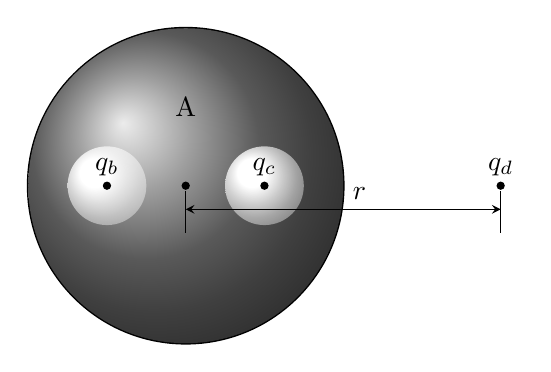
\begin{tikzpicture}
                    \begin{scope}[blend group=screen]
                        \filldraw[ball color=gray] (0,0) circle(2) node[above]{A};
                        \fill[ball color=white!50] (1,0) circle(0.5);
                        \fill[ball color=white!50] (-1,0) circle(0.5);
                    \end{scope}
                    \node at (0,1) {A};
                    \fill (0,0) circle(1.5pt);
                    \fill (1,0) circle(1.5pt) node[above]{\(q_c\)};
                    \fill (-1,0) circle(1.5pt) node[above]{\(q_b\)};
                    \fill (4,0) circle(1.5pt) node[above]{\(q_d\)};
                    \draw (0,-2pt) -- (0,-0.6);
                    \draw (4,-2pt) -- (4,-0.6);
                    \draw[stealth-stealth] (0,-0.3) -- node[above right]{\(r\)} (4,-0.3);
                \end{tikzpicture}
                \caption*{\ref{itm:6} 题图}
            \end{minipage}
            \begin{minipage}[b]{0.4\textwidth}
                \centering
                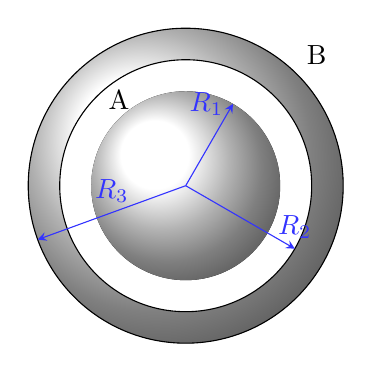
\begin{tikzpicture}
                    \filldraw[ball color=white] (0,0) circle(2);
                    \filldraw[fill = white] (0,0) circle(1.6);
                    \fill[ball color=white] (0,0) circle(1.2);
                    \node[above right] at (45:2){B};
                    \node[above] at (135:1.2){A};
                    \draw[blue!80,-stealth] (0,0) -- (60:1.2) node[left]{\(R_1\)};
                    \draw[blue!80,-stealth] (0,0) -- (330:1.6) node[above]{\(R_2\)};
                    \draw[blue!80,-stealth] (0,0) -- node[above]{\(R_3\)} (200:2);
                \end{tikzpicture}
                \caption*{\ref{itm:10} 题图}
            \end{minipage}
        \end{figure}
    
    \item[6-8] 一个导体球半径为\(R_1\),外罩一个半径为\(R_2\)的同心薄导体球壳,外球壳所带总电荷
        为\(Q\),而内球的电势为\(V_0\)。求此系统的电势和电场分布。
    
    \item[\mlabel{itm:10}{6-10}] 如图所示,在一个半径为\(R_1=6.0\,\mathrm{cm}\)的金属球A外面套一个
        同心的金属球壳B。已知球壳B的内、外半径分别为\(R_2=8.0\,\mathrm{cm},R_3=10.0\,\mathrm{cm}\)。
        设球A带有总电荷\(Q_{\mathrm{A}}=3.0\times 10^{-8}\,\mathrm{C}\),球壳B带有总电荷\(Q_{\mathrm{B}}=2.0\times 10^{-8}\,\mathrm{C}\)。
        (1)求球壳B内、外表面上所带的电荷以及球A和球壳B的电势;\mbox{*(2)}将球壳B接地后断开,再把金属球A接地,
        求金属球A和球壳B内、外表面上所带的电荷以及球A和球壳B的电势。
    
    \item[\mlabel{itm:11}{6-11}] 同轴传输线由长直圆柱形导线和同轴的导体圆筒构成,导线的半径为\(R_1\),电势为\(V_1\),
        圆筒的半径为\(R_2\),电势为\(V_2\),如图所示。试求他们之间距离轴线\(r\)处(\(R_1<r<R_2\))
        的电场强度。
        \begin{figure}[htb]
            \centering
            \begin{minipage}[b]{0.4\textwidth}
                \centering
                \begin{tikzpicture}
                    \shade[draw=black,left color = white,right color=gray] (0:2 and 1) arc (0:180:2 and 1) 
                        -- +(0,-4) arc (180:360:2 and 1) --cycle;
                    \shade[draw=black,left color = white,right color=gray,path fading=fade left] (0:1 and 0.5) arc (0:180:1 and 0.5) 
                        -- +(0,-4) arc (180:360:1 and 0.5) --cycle;
                    \draw[draw=black] (180:2 and 1) arc (180:360:2 and 1) 
                        --+(0,-4) arc (360:180:2 and 1) -- cycle;
                    \draw (-1,0) -- (-1,-0.86);
                    \draw (1,0) -- (1,-0.86);
                    \filldraw[draw=black, fill=lightgray] (0,0) ellipse (1 and 0.5);
                    \draw[blue!80,-stealth] (0,0) -- node[above]{\(R_1\)} (30:1 and 0.5);
                    \draw[blue!80,-stealth] (0,0) -- (330:2 and 1) node[above left]{\(R_2\)};
                    \node[left] at (180:1 and 0.5) {\(V_1\)};
                    \node[below left] at (180:2 and 1) {\(V_2\)};
                \end{tikzpicture}
                \caption*{\ref{itm:11} 题图}
            \end{minipage}
            \begin{minipage}[b]{0.4\textwidth}
                \centering
                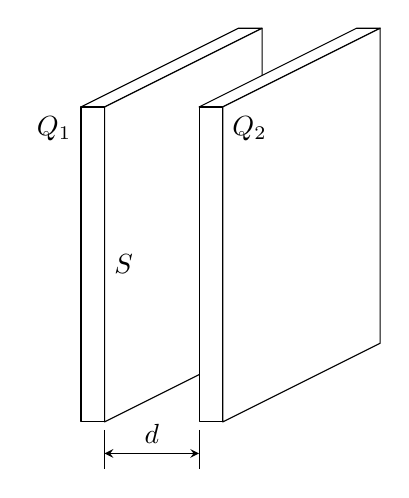
\begin{tikzpicture}
                    \filldraw[fill=white,draw=black,join=round] (0,0) -- (2,1) -- (1.7,1) -- (-0.3,0) -- cycle;
                    \filldraw[fill=white,draw=black,join=round] (0,0) -- (0,-4) -- (-0.3,-4) -- (-0.3,0) --cycle;
                    \filldraw[fill=white,draw=black,join=round] (0,0) -- (2,1) -- +(0,-4) -- (0,-4) --cycle;
                    \begin{scope}[xshift=1.5cm]
                        \filldraw[fill=white,draw=black,join=round] (0,0) -- (2,1) -- (1.7,1) -- (-0.3,0) -- cycle;
                        \filldraw[fill=white,draw=black,join=round] (0,0) -- (0,-4) -- (-0.3,-4) -- (-0.3,0) --cycle;
                        \filldraw[fill=white,draw=black,join=round] (0,0) -- (2,1) -- +(0,-4) -- (0,-4) --cycle;
                    \end{scope}
                    \node[below left] at (-0.3,0) {\(Q_1\)};
                    \node[below right] at (1.5,0) {\(Q_2\)};
                    \node[right] at (0,-2) {\(S\)};
                    \draw (0,-4.1) -- (0,-4.6);
                    \draw (1.2,-4.1) -- (1.2,-4.6);
                    \draw[stealth-stealth] (0,-4.4) -- node[above]{\(d\)} (1.2,-4.4);
                \end{tikzpicture}
                \caption*{\ref{itm:13} 题图}
            \end{minipage}
        \end{figure}
    \item[\mlabel{itm:13}{6-13}] 如图所示,两块分别带电荷为\(Q_1\)、\(Q_2\)的导体平板平行相对放置,假设导体平板
        面积为\(S\),两块导体平板间距为\(d\),并且\(\sqrt{S}\gg d\)。试证明:(1)相向的两面,电荷面密度大小相等
        符号相反;(2)相背的两面,电荷面密度大小相等符号相同。
    
    \item[\mlabel{itm:16}{6-16}] 如图所示,在真空中将半径为\(R\)的金属球接地,在与球心\(O\)相距为\(r\)(\(r<R\))
        处放置一点电荷\(q\),不计接地导线上电荷的影响,求金属球表面上的感应电荷。
        
        \begin{figure}[htb]
            \centering
            \begin{minipage}[b]{0.4\textwidth}
                \centering
                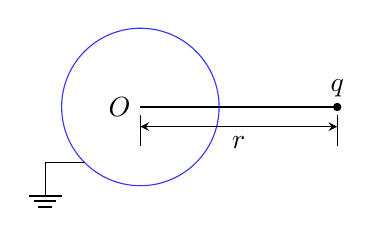
\begin{tikzpicture}
                    \draw[blue!80] (0,0) circle (1);
                    \draw (0,0) node[left]{\(O\)} -- (2.5,0) node[above]{\(q\)};
                    \draw (0,-0.1) -- (0,-0.5);
                    \draw (2.5,-0.1) -- (2.5,-0.5);
                    \fill (2.5,0) circle (1.5pt);
                    \draw[stealth-stealth] (0,-0.25) -- node[below]{\(r\)} (2.5,-0.25);
                    \draw (225:1) -- +(-0.5,0) node[ground,thin]{}; 
                \end{tikzpicture}
                \caption*{\ref{itm:16} 题图}
            \end{minipage}
        \end{figure}

    \item[6-19] 两根输电导线的半径为3.26\,mm,两导线中心相距0.50\,m。导线位于地面上空很高处,
        因而大地的影响可以忽略,求输电导线单位长度的电容。
    
    \item[\mlabel{itm:20}{6-20}] 电容式计算机键盘的每一个键下面连接一小块金属片,金属片与底板上的另一
        块金属片间保持一定的空气间隙,构成一小电容器(如图所示)。当按键按下时电容发生变化,并通过与之
        相连的电子线路向计算机发出相应的信号。设金属片面积为\(50.0\,\mathrm{mm}^2\),两金属片之间的距离为0.600\,mm。
        如果电路能检测出的电容变化量是0.250\,pF,那么按键需要按下多大的距离才能给出必要的信号?
        
        \begin{figure}[htb]
            \centering
            \begin{minipage}[b]{0.4\textwidth}
                \centering
                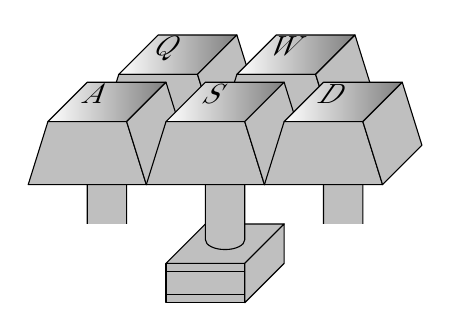
\begin{tikzpicture}
                    \newcommand{\key}[2]
                    {
                        \shade[join = round, draw = black,left color=white,right color = gray] #1 -- ++(1,0) -- ++(0.5,0.5) -- ++(-1,0) -- cycle;
                        \filldraw[join = round, draw = black, fill = lightgray] #1 -- ++(1,0) -- ++(0.25,-0.8) -- ++(-1.5,0) -- cycle;
                        \filldraw[join = round, draw = black, fill = lightgray] #1++(1,0) -- ++(0.5,0.5) --  ++(0.25,-0.8) -- ++(-0.5,-0.5) -- cycle;
                        \node[below,xslant=0.7,] at ($ #1 + (0.8,0.6) $) {#2};
                    }
                    \key{(-0.6,0.6)}{Q};
                    \key{(0.9,0.6)}{W};
                    \filldraw[join = round, draw = black, fill = lightgray] (0,-1.8) -- ++(1,0) -- ++(0.5,0.5) -- ++(-1,0) -- cycle;
                    \filldraw[join = round, draw = black, fill = lightgray] (0.5,-0.5) -- (1,-0.5) -- (1,-1.5) arc (360:180:0.25 and 0.125) -- cycle;
                    \filldraw[join = round, draw = black, fill = lightgray] (0,-1.8) -- ++(1,0) -- ++(0,-0.5) -- ++(-1,0) -- cycle; 
                    \filldraw[join = round, draw = black, fill = lightgray] (0,-1.9) -- ++(1,0) -- ++(0,-0.3) -- ++(-1,0) -- cycle; 
                    \filldraw[join = round, draw = black, fill = lightgray] (0,-1.8)++(1,0) -- ++(0.5,0.5) -- ++(0,-0.5) -- ++(-0.5,-0.5) -- cycle; 
                    \filldraw[join = round, draw = black, fill = lightgray] (2,-0.5) -- (2.5,-0.5) -- (2.5,-1.5) arc (360:180:0.25 and 0.125) -- cycle;
                    \fill[white] (2.6,-1.3) rectangle (1.9,-1.8);
                    \filldraw[join = round, draw = black, fill = lightgray] (-1,-0.5) -- (-0.5,-0.5) -- (-0.5,-1.5) arc (360:180:0.25 and 0.125) -- cycle;
                    \fill[white] (-1.1,-1.3) rectangle (-0.4,-1.8);
                    \key{(-1.5,0)}{A};
                    \key{(0,0)}{S};
                    \key{(1.5,0)}{D};
                \end{tikzpicture}
                \caption*{\ref{itm:20} 题图}
            \end{minipage}
            \begin{minipage}[b]{0.4\textwidth}
                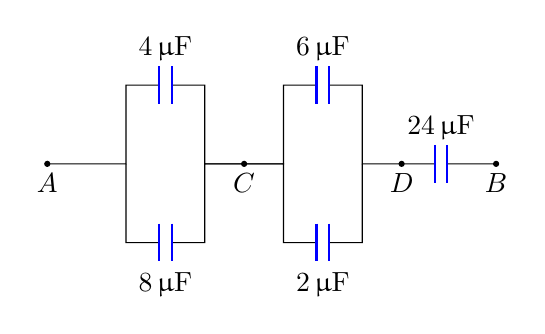
\begin{tikzpicture}
                    \ctikzset{bipoles/length=.8cm} 
                    \draw (0,0) node[below]{\(A\)} to[short, *-] ++(1,0) -- ++(0,1) to[C=\(4\,\mathrm{\upmu F}\),color=blue] ++(1,0) -- ++(0,-1) to[short, -*] ++(0.5,0) node[below]{\(C\)} -- ++(0.5,0) -- ++(0,1) 
                        to[C=\(6\,\mathrm{\upmu F}\),color=blue] ++(1,0) -- ++(0,-1) to[short, -*] ++(0.5,0) node[below]{\(D\)} to[C=\(24\,\mathrm{\upmu F}\),color=blue] ++(1,0) 
                        to[short, -*] ++(0.2,0) node[below]{\(B\)};
                    \draw (1,0) -- ++(0,-1) to[C,l_=\(8\,\mathrm{\upmu F}\),color=blue] ++(1,0) -- ++(0,1) -- ++(1,0) -- ++(0,-1) to[C,l_=\(2\,\mathrm{\upmu F}\),color=blue] ++(1,0) -- ++(0,1) ;
                \end{tikzpicture}
                \caption*{\ref{itm:22} 题图}
            \end{minipage}
        \end{figure}

    \item[\mlabel{itm:22}{6-22}] 如图所示,在点\(A\)和点\(B\)之间有5个电容器。
        (1)求\(A\)、\(B\)两点之间的等效电容;
        (2)若\(A\)、\(B\)之间的电势差为12\,V,求\(U_{AC}\)、\(U_{CD}\)和\(U_{DB}\)。
    
    \item[6-24] 一片二氧化钛晶片的面积为\(1.0\,\mathrm{cm^2}\),厚度为0.10\,mm,把平行平板电容器的两极板
        紧贴在晶片两侧。(1)求电容器的电容;(2)当在电容器的两极板上加12\,V电压时,极板上的电荷为多少?
        此时自由电荷和极化电荷的面密度各为多少?(3)求电容器内的电场强度。
    
    \item[\mlabel{itm:25}{6-25}] 如图所示,半径\(R=0.10\,\mathrm{m}\)的导体球带有电荷\(Q=1.0\times 10^{-8}\mathrm{C}\),导体球外
        有两层均匀介质,一层介质的\(\varepsilon_r=5.0\),厚度为\(d=0.10\,\mathrm{m}\),另一层介质为空气,充满其余空间。求:
        (1)离球心为\(r=5\,\mathrm{cm},15\,\mathrm{cm},25\,\mathrm{cm}\)处的电位移\(\bm{D}\)和电场强度\(\bm{E}\);
        (2)离球心为\(r=5\,\mathrm{cm},15\,\mathrm{cm},25\,\mathrm{cm}\)处的电势;
        (3)极化电荷面密度。
        \begin{figure}[htb]
            \centering
            \begin{minipage}[b]{0.4\textwidth}
                \centering
                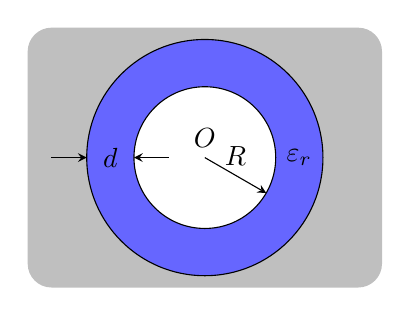
\begin{tikzpicture}[scale=1.5]
                    \fill[lightgray,rounded corners=2ex] (-1.5,1.1) rectangle (1.5,-1.1);
                    \filldraw[fill=blue!60,draw=black] (0,0) circle(1);
                    \filldraw[fill=white,draw=black] (0,0) circle(0.6);
                    \draw[stealth-] (180:1) -- +(-0.3,0);
                    \draw[stealth-] (180:0.6) -- +(0.3,0);
                    \draw[draw opacity=0] (180:0.6) -- (180:1) node[midway]{\(d\)};
                    \node at (0:0.8) {\(\varepsilon_r\)};
                    \draw[-stealth] (0,0) node[above]{\(O\)} -- node[above]{\(R\)} (-30:0.6);
                \end{tikzpicture}
                \caption*{\ref{itm:25} 题图}
            \end{minipage}
            \begin{minipage}[b]{0.4\textwidth}
            \end{minipage}
        \end{figure}
    
    \item[\mlabel{itm:28}{6-28}] 两块面积为\(S\)的导体板构成一平板电容器,导体极板间距离为\(d\)。将平板电容器两极板接到
        电压为\(U\)的电源上,接通电源后在导体极板间的一半插入电容率为\(\varepsilon\)的电介质,略去边缘效应。
        (1)试比较\(A\)、\(B\)两点的电场强度各为未插入电介质时的多少倍?
        (2)假如电容器充满电后,先断开电源,再在导体极板间的一半插入电介质,则结果又将如何?
        
        \begin{figure}[htb]
            \centering
            \begin{minipage}[b]{0.4\textwidth}
                \centering
                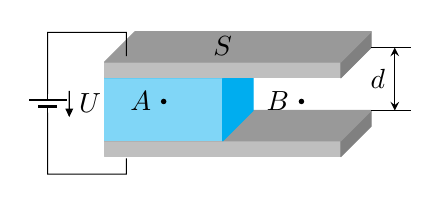
\begin{tikzpicture}[
                    dot/.style = {circle, fill, minimum size=#1,
                                  inner sep=0pt, outer sep=0pt},
                    dot/.default = 6pt] 
                    \ctikzset{bipoles/length=.8cm} 
                    \cube{(0,0,0)}{3}{0.2}{1}{gray};
                    \cube{(-1.5,0.8,0)}{1.5}{0.8}{1}{cyan};
                    \cube{(0,1,0)}{3}{0.2}{1}{gray};
                    \draw (-2.8,1,-0.2) -- ++ (0,0.3,0) -- ++(-1,0,0) to[battery1=\(U\)] ++(0,-1.8,0) -- ++(1,0,0) -- ++(0,0.2,0);
                    \node at (-1.5,1.2,0) {\(S\)};
                    \node[dot=2pt,label=left:\(A\)] at (-2.25,0.5,0) {};
                    \node[dot=2pt,label=left:\(B\)] at (-0.5,0.5,0) {};
                    \draw (0,0,-1) -- +(0.5,0,0);
                    \draw (0,0.8,-1) -- +(0.5,0,0);
                    \draw[stealth-stealth] (0.3,0,-1) -- node[left]{\(d\)} +(0,0.8,0);
                \end{tikzpicture}
                \caption*{\ref{itm:28} 题图}
            \end{minipage}
            \begin{minipage}[b]{0.4\textwidth}
                \centering
                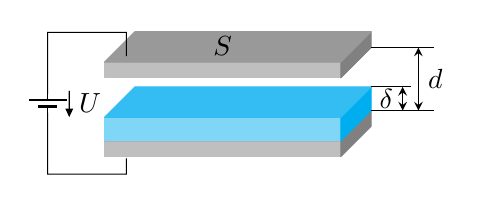
\begin{tikzpicture}
                    \ctikzset{bipoles/length=.8cm} 
                    \cube{(0,0,0)}{3}{0.2}{1}{gray};
                    \cube{(0,0.3,0)}{3}{0.3}{1}{cyan};
                    \cube{(0,1,0)}{3}{0.2}{1}{gray};
                    \draw (-2.8,1,-0.2) -- ++ (0,0.3,0) -- ++(-1,0,0) to[battery1=\(U\)] ++(0,-1.8,0) -- ++(1,0,0) -- ++(0,0.2,0);
                    \node at (-1.5,1.2,0) {\(S\)};
                    \draw (0,0,-1) -- +(0.8,0,0);
                    \draw (0,0.8,-1) -- +(0.8,0,0);
                    \draw (0,0.3,-1) -- +(0.5,0,0);
                    \draw[stealth-stealth] (0.6,0,-1) -- node[right]{\(d\)} +(0,0.8,0);
                    \draw[stealth-stealth] (0.4,0,-1) -- node[left]{\(\delta\)} +(0,0.3,0);
                \end{tikzpicture}
                \caption*{\ref{itm:29} 题图}
            \end{minipage}
        \end{figure}

    \item[\mlabel{itm:29}{6-29}] 如图所示,一个空气平板电容器的极板面积为\(S\),间距为\(d\)。现将该电容器接到电压为\(U\)
        的电源上充电,当(1)充足电后,(2)然后平行插入一块面积相同,厚度为\(\delta(\delta<d)\)、相对电容率为\(\varepsilon_r\)
        的电介质板,(3)将上述电介质换为同样大小的导体板时,分别求极板上的电荷\(Q\)、极板间的电场强度\(\bm{E}\)和电容器的电容\(C\)。
    
    \item[6-37] 某介质的相对电容率\(\varepsilon_r=2.8\),击穿电场强度为\(18\times 10^6\,\mathrm{V\cdot m^{-1}}\)。如果用它来作
        平板电容器的电介质,要制作电容为\(0.047\,\upmu\mathrm{F}\),而耐压为4.0\,kV的电容器,它的极板面积至少要多大?
    
    \item[*6-40] 一个空气平板电容器,极板面积为\(S\),极板间距为\(d\),充电至带电\(Q\)后与电源断开,然后用外力缓缓地将两极板间距
        拉开到\(2d\)。求:(1)电容器能量的改变;(2)此过程中外力所做的功,并讨论此过程中的功能转化关系。
    
    \item \label{itm:s1} \(ABC\)是三块平行金属板,面积均为\(S\);\(AC\)板相距为\(d\);\(BC\)板相距为\(2d\);\(AB\)两板都接地(如图所示),
        \(C\)板带正点荷\(Q\),不计边缘效应,求:\\
        (1)求\(A\)板和\(B\)板上的感应电荷\(Q_A\),\(Q_B\)及\(C\)板的电势\(V_C\);\\
        (2)若在\(CB\)两板之间充以相对介电常数为\(\varepsilon_r\)的均匀电介质,再求\(A\)板和\(B\)板上的感应电荷\(Q_A^\prime\)、\(Q_B^\prime\)及\(C\)板的电势\(V_C^\prime\)。
        \begin{figure}[htb]
            \centering
            \begin{minipage}[b]{0.4\textwidth}
                \centering
                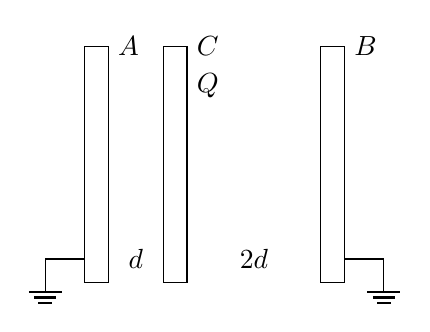
\begin{tikzpicture}
                    \draw (0,0) rectangle (0.3,3) node[right]{\(A\)};
                    \draw (1,0) rectangle (1.3,3) node[right]{\(C\)};
                    \draw (3,0) rectangle (3.3,3) node[right]{\(B\)};
                    \node[right] at (1.3,2.5){\(Q\)};
                    \node at (0.65,0.3){\(d\)};
                    \node at (2.15,0.3){\(2d\)};
                    \draw (0,0.3) -- +(-0.5,0) node[ground]{};
                    \draw (3.3,0.3) -- +(0.5,0) node[ground]{};
                \end{tikzpicture}
                \caption*{\ref{itm:s1} 题图}
            \end{minipage}
            \begin{minipage}[b]{0.4\textwidth}
                \centering
                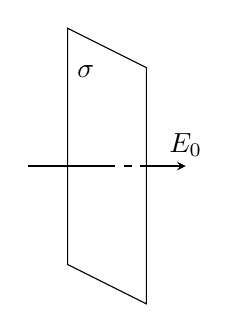
\begin{tikzpicture}
                    \draw[yslant=-0.5] (-0.5,1.5) rectangle (0.5,-1.5);
                    \draw (-1,0) -- (0,0);
                    \draw[dashed] (0,0) -- (0.5,0);
                    \node[right] at (-0.5,1.2) {\(\sigma\)};
                    \draw[-stealth] (0.5,0) -- (1,0) node[above]{\(E_0\)};
                \end{tikzpicture}
                \caption*{\ref{itm:s2} 题图}
            \end{minipage}
        \end{figure}
    
    \item \label{itm:s2} 将一块两面总电荷面密度为\(\sigma\)的无限大带电金属平板置于与板面垂直的匀强电场\(E_0\)中,如题图所示,
        试求金属板与电场垂直的两个面上电荷的分布以及金属板外的场强分布。
    
    \item \label{itm:s3} 如图所示,一平行板电容器两极板的面积都是\(S\),相距为\(d\),今在其间平行地插入厚度为\(t\)、
        电容率为\(\varepsilon\)的均匀介质,其面积为\(\frac{S}{2}\),设两板分别带电荷\(Q\)和\(-Q\),略去边缘效应,
        求两板电势差\(U\)、电容\(C\)和介质的极化电荷面密度\(\sigma^\prime\)。
        \begin{figure}[htb]
            \centering
            \begin{minipage}[b]{0.4\textwidth}
                \centering
                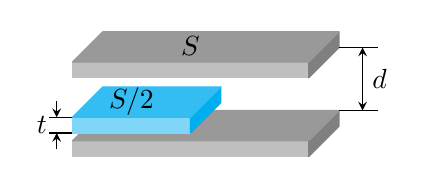
\begin{tikzpicture}
                    \ctikzset{bipoles/length=.8cm} 
                    \cube{(0,0,0)}{3}{0.2}{1}{gray};
                    \cube{(-1.5,0.3,0)}{1.5}{0.2}{1}{cyan};
                    \cube{(0,1,0)}{3}{0.2}{1}{gray};
                    \node at (-1.5,1.2,0) {\(S\)};
                    \node at (-2.25,0.5,0) {\(S/2\)};
                    \draw (0,0,-1) -- +(0.5,0,0);
                    \draw (0,0.8,-1) -- +(0.5,0,0);
                    \draw (-3,0.1,0) -- +(-0.3,0,0);
                    \draw (-3,0.3,0) -- +(-0.3,0,0);
                    \draw[stealth-stealth] (0.3,0,-1) -- node[right]{\(d\)} +(0,0.8,0);
                    \draw[draw opacity=0] (-3.2,0.1,0) -- node[left]{\(t\)} +(0,0.2,0);
                    \draw[stealth-] (-3.2,0.1,0) -- +(0,-0.2,0);
                    \draw[stealth-] (-3.2,0.3,0) -- +(0,0.2,0);
                \end{tikzpicture}
                \caption*{\ref{itm:s3} 题图}
            \end{minipage}
            \begin{minipage}[b]{.4\textwidth}
                \centering 
                \begin{tikzpicture}
                    \ctikzset{bipoles/length=.8cm} 
                    \draw (0,0) -- ++(1,0) -- ++(0,0.8) to[C=\(C_2\),color=cyan] ++(1,0) to[C=\(C_3\),color=cyan] ++(1,0) -- ++(0,-0.8) -- ++(1,0);
                    \draw (1,0)-- ++(0,-0.8) to[C=\(C_1\),color=cyan] ++(2,0) -- ++(0,0.8);
                \end{tikzpicture}
                \caption*{\ref{itm:s4} 题图}
            \end{minipage}
        \end{figure}
    
    \item \label{itm:s4} 有三个电容分别为\(C_1\)、\(C_2\)、\(C_3\)的电容器,先将\(C_1\)充电至\(U_0\),然后将三个电容串接成闭合回路,
        如图所示。试求各电容上的电量及电压。

    \item \label{itm:s5} 两个同心导体球壳,外球壳的内半径为5\,cm,内球壳的外半径可自由选择,两球壳之间充满各向同性的均匀电介质。
        设电介质的击穿场强为\(2.0\times 10^7\,\mathrm{V\cdot m^{-1}}\)。试求该电容器所能承受的最大电压。
        % \begin{figure}[htb]
        %     \centering
        %     \begin{minipage}[b]{0.4\textwidth}
        %         \centering
        %         \begin{tikzpicture}
        %             \filldraw[ball color=gray] (0,0) circle(1.5);
        %             \filldraw[ball color=white] (0,0) circle(1);
        %         \end{tikzpicture}
        %         \caption*{\ref{itm:s3} 题图}
        %     \end{minipage}
        % \end{figure}
\end{enumerate}
\end{document} 